\chapter{Implementacja aplikacji}
%
\section{Architektura aplikacji webowej}
Aplikacja składa się z następujących elementów (rys. \ref{fig:systemarchitecturediagram}):
\begin{itemize}
\item MongoDB - baza danych;
\item Redis - przechowywanie JWT tokenów po wylogowaniu;
\item Go - część serwerowa napisana w języku Go;
\item Android - aplikacja mobilna;
\item Docker - kontener dla wdrożenia aplikacji webowej;
\end{itemize}
    \begin{figure}[ht]
    \centering
        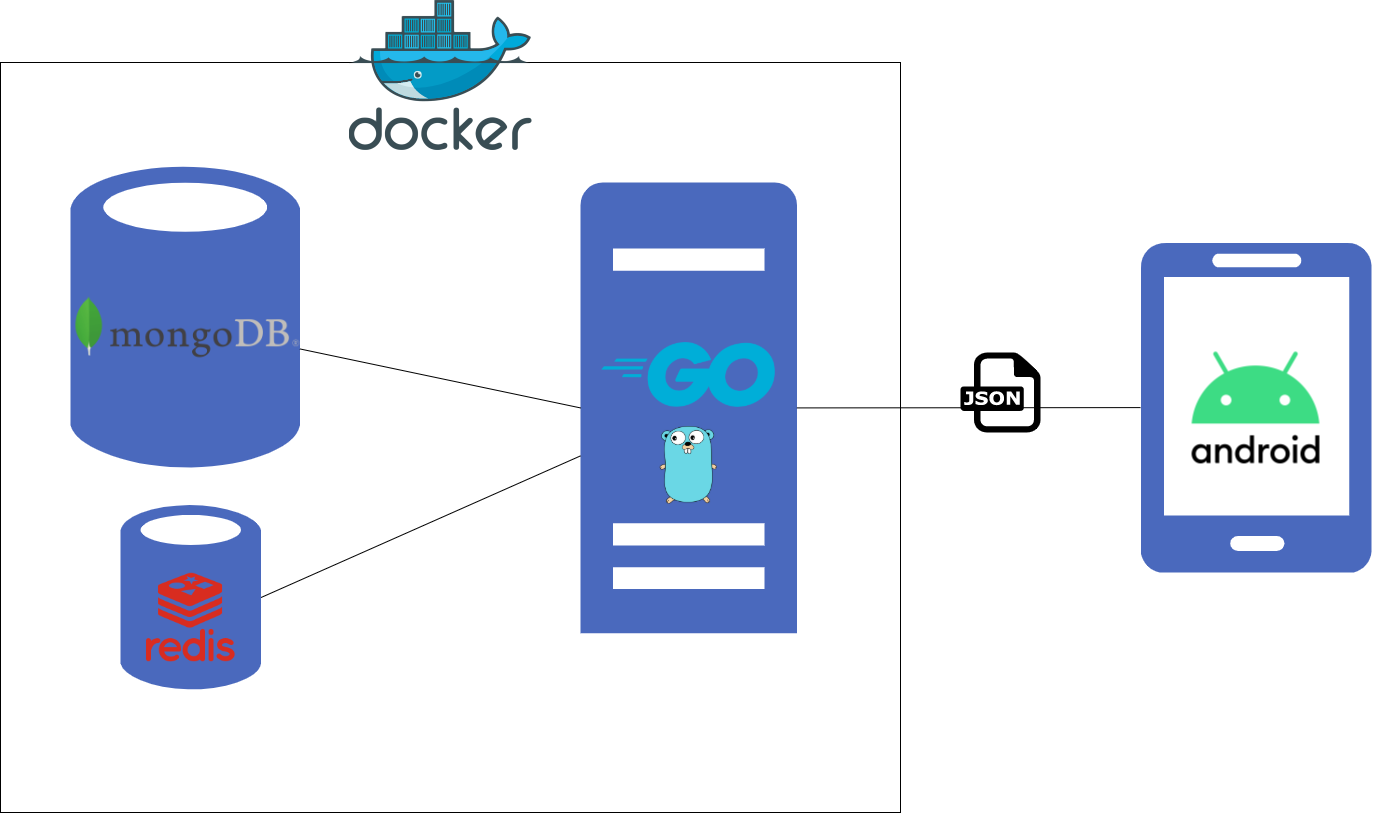
\includegraphics[width=0.8\linewidth]{rys03/system_architecture_diagram.png}
    \caption{architektura systemu \cite{diagrams_net}}
    \label{fig:systemarchitecturediagram}
\end{figure}
\section{Model bazy danych}
W systemie wykorzystano dwie nierelacyjne bazy danych: MongoDB i Redis.
MongoDB jest przeznaczona do przechowywania danych aplikacji.
Redis wykorzystuje się tylko do czasowego przechowywania tokenów.

% 
\paragraph{MongoDB\newline}
% TO DO: proszę stosować czcionkę maszynową do kodu źródłowego, nazw zmiennych i klas, nazw plików itp.
% DONE: dziękuję, po prostu nie wiedziałem jak to zrobić z nazwami.
% TO DO: aby zdefiniować zawartość plików json można posłużyć się specyfikacją json schema : https://json-schema.org/
% TO DO: prawdopodobnie dokumenty w MongoDB powstają poprzez mapowanie z obiektów dostępnych w języku programowania,
%  jeśli tak jest, to należy o tym powiedzieć (w opisie implementacji można pokazać diagram klas zawierających odpowiednie pola)
% TO VERIFY: ten json jest wycinkiem z konsoli bazy danych ,,mongo'' po wprowadzeniu odpowiedniego zapytania (,,db.nazwakolekcji.find({});''), różni się od odpowiedzi, które otrzymałem w tej konsoli tym, że sformatowano do czytelnego tekstu, a nie wszystko w jednej linii.
Baza danych składa się z dwóch kolekcji: \texttt{station} i \texttt{user}. Kolekcja \texttt{user} składa się z następujących pól:
\texttt{
    \begin{itemize}
        \item \_id : ObjectId(String)
        \item user\_name : String
        \item email : String
        \item password : String
        \item Model : Object :
        \begin{itemize}
            \item create\_at : ISODate
            \item update\_at : ISODate
            \item delete\_at : ISODate
        \end{itemize}
    \end{itemize}
}

Przykład encji:
\begin{lstlisting}[basicstyle=\tiny\ttfamily]
    {
        "_id":ObjectId("5fb93e4b721953b7c60983c6"),
        "user_name":"newtest",
        "email":"newtest@test.test",
        "password":"$2a$04$o0WfZvdk4WUpsct.BH3zw.3MFJFmUuLe8VjJx2OeyxtZuBliMOrl.",
        "model":{
            "create_at":ISODate("2020-11-21T16:20:27.044Z"),
            "update_at":ISODate("2020-11-21T16:20:27.044Z"),
            "delete_at":ISODate("0001-00-00T00:00:00Z")
        }
    }
\end{lstlisting}

Kolekcja \texttt{station} składa się z następujących pól:
\texttt{
    \begin{itemize}
        \item \_id : String
        \item station\_name : String
        \item owner\_id : String
        \item rating : Double
        \item latitude : Double
        \item longitude : Double
        \item description : String
        \item comments : Array :
        \begin{itemize}
            \item \_id : String
            \item user\_id : String
            \item user\_name : String
            \item text : String
            \item rating : Double
            \item model : Object :
            \begin{itemize}
                \item create\_at : ISODate
                \item update\_at : ISODate
                \item delete\_at : ISODate
            \end{itemize}
        \end{itemize}
        \item model : Object :
        \begin{itemize}
            \item create\_at : ISODate
            \item update\_at : ISODate
            \item delete\_at : ISODate
        \end{itemize}
    \end{itemize}
}

Przykład encji:
\begin{lstlisting}[basicstyle=\tiny\ttfamily]
    {
        "_id":ObjectId("5fca6f81bb37f04ad438c1a5"),
        "station_name":"Station Name",
        "owner_id":"5fb828babe10c57ba70d49cd",
        "rating":3.6666666666666665,
        "description":"description",
        "latitude":57.12662933894774,
        "longitude":14.208925142884254,
        "model":{
            "create_at":ISODate("2020-12-04T17:18:57Z"),
            "update_at":ISODate("2020-12-04T17:20:55Z"),
            "delete_at":ISODate("0001-00-00T00:00:00Z")
        },
        "comments":[
            {
                "_id":"5fca6ff7bb37f04ad438c1a8",
                "user_id":"5fb828babe10c57ba70d49cd",
                "user_name":"test",
                "text":"  Comment 3",
                "rating":5,
                "model":{
                    "create_at":ISODate("2020-12-04T17:20:55Z"),
                    "update_at":ISODate("2020-12-04T17:20:55Z"),
                    "delete_at":ISODate("0001-00-00T00:00:00Z")
                }
            },
            {
                "_id":"5fca6fe5bb37f04ad438c1a7",
                "user_id":"5fb828babe10c57ba70d49cd",
                "user_name":"test",
                "text":" Comment 2",
                "rating":3,
                "model":{
                    "create_at":ISODate("2020-12-04T17:20:37Z"),
                    "update_at":ISODate("2020-12-04T17:20:37Z"),
                    "delete_at":ISODate("0001-00-00T00:00:00Z")
                }
            },
            {
                "_id":"5fca6fb8bb37f04ad438c1a6",
                "user_id":"5fb828babe10c57ba70d49cd",
                "user_name":"test",
                "text":"Comment 1",
                "rating":3,
                "model":{
                    "create_at":ISODate("2020-12-04T17:19:52Z"),
                    "update_at":ISODate("2020-12-04T17:19:52Z"),
                    "delete_at":ISODate("0001-00-00T00:00:00Z")
                }
            }
        ]
    }
\end{lstlisting}

% 
\paragraph{Redis\newline}
Baza danych Redis wykorzystana tylko dla przechowywania tokenów użytkowników, które już wylogowane, ponieważ jedną z wad JWT tokenów jest to, że wygenerowany token nie można zrobić nieważny, dopóki nie skończy się czas jego działania.
Redis częściowo eliminuje ten problem.

W nim przechowuje się para klucz - wartość, pewny czas. Po upływie tego czasu zapis automatycznie jest usuwany.
Dla szybkiego wyszukiwania encja wygląda w następujący sposób: \texttt{token}, \texttt{token}. To pozwala często wylogować użytkowniku, ale zajmuje więcej miejsca niż encja typu: \texttt{user\_id}, \texttt{token}.

\section{Implementacja części serwerowej}
% 
\subsection{Struktura RestApi}
% 
\subsubsection{Narzędzia, technologie, biblioteki}
Do stworzenia serwerowej części aplikacji użyto następujących technologii:
\begin{itemize}
\item Visual Studio Code - środowisko programistyczne;
\item Go - język programowania;
\item Go Modules - system zarządzania zależnościami;
\item gorilla/mux - Router mapuje przychodzące żądania na listę zarejestrowanych tras i wywołuje moduł obsługi tego żądania, który odpowiada URL (ang. \textit{Uniform Resource Locator}) adresowi;
\item sirupsen/logrus - rejestrator strukturalny;
\item mongo-driver - sterowanie MongoDB z języka Go;
\item go-redis/redis - sterowanie Redis z języka Go;
\item dgrijalva/jwt-go - realizacja JWT w języku Go;
\item crypto/bcrypt - realizuje algorytm haszowania bcrypt Provosa i Mazierao;
\item go-ozzo/ozzo-validation - pakiet wspomagający na walidację danych;
\item yaml.v2 - implementuje obsługę YAML (ang. \textit{Yet Another Markup Language});
\item google/uuid - sprawdza i generuje UUID (ang. \textit{universally unique identifier});
\end{itemize}

% 
\subsubsection{Struktura plików RestApi}
Na rysunku \ref{fig:backend_file_structure} została przedstawiona struktura plików części serwerowej. Obok plików, niezbędnych do działania aplikacji, znajdują się pliki pozwalające na prowadzenie testów jednostkowych. Te pliki mają nazwę w postaci \texttt{*\_test.go}.
% TO DO: proszę poukładać obrazki ze strukturami plików obok siebie (pojedynczo zajmują za dużo miejsca)
% TO VERIFY:
\begin{figure}[ht]
\centering
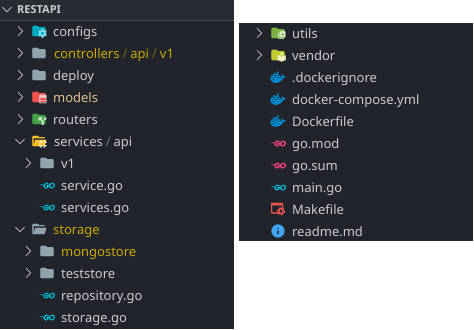
\includegraphics[width=0.25\linewidth]{rys03/backend_file_structure.png}
\caption{Struktura plików}
\label{fig:backend_file_structure}
\end{figure}
\begin{figure}[ht]
	\centering
    \begin{tabular}{@{}rl@{\hspace{3mm}}rl@{\hspace{3mm}}rl@{}}
        a) & \vtop{\vskip-2ex\hbox{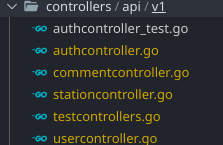
\includegraphics[width=0.25\linewidth]{rys03/controllers.png}}} &
        b) & \vtop{\vskip-2ex\hbox{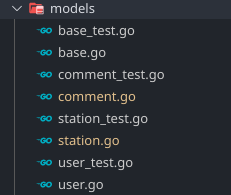
\includegraphics[width=0.25\linewidth]{rys03/model.png}}} &
        c) & \vtop{\vskip-2ex\hbox{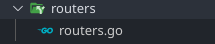
\includegraphics[width=0.25\linewidth]{rys03/routers.png}}}
    \end{tabular}
    \caption{Struktura plików: a) kontrolery, b) modeli danych, c) routery.}
    \label{fig:backend_file_structure_1}
\end{figure}
\begin{figure}[ht]
	\centering
    \begin{tabular}{@{}rl@{\hspace{3mm}}rl@{\hspace{3mm}}rl@{}}
        a) & \vtop{\vskip-2ex\hbox{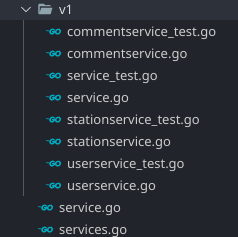
\includegraphics[width=0.25\linewidth]{rys03/services.png}}} &
        b) & \vtop{\vskip-2ex\hbox{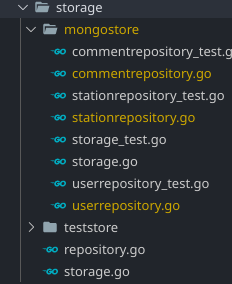
\includegraphics[width=0.25\linewidth]{rys03/storage.png}}} &
        c) & \vtop{\vskip-2ex\hbox{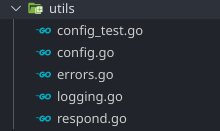
\includegraphics[width=0.25\linewidth]{rys03/utils.png}}}
    \end{tabular}
    \caption{Struktura plików: a) serwisy, b) wszpółdziałania z bazą danych, c) narzędzia.}
    \label{fig:backend_file_structure_2}
\end{figure}

Katalog \texttt{config} zawiera pliki konfiguracyjne. W katalogu \texttt{controllers} (rys.~\ref{fig:backend_file_structure_1}a) znajdują się kontrolery, które są wykorzystywanie do połączenia poziomu serwisów z punktami końcowymi serwera (ang.~\emph{endpoints}).

Do katalogu \texttt{deploy} jest kompilowana aplikacja przy uruchomieniu \texttt{Makefile}.

Katalog \texttt{models}(rys. \ref{fig:backend_file_structure_1}b) zawiera modeli danych do przechowywania w bazie danych oraz do przekazania do interfejsu użytkownika.

Katalog \texttt{routers} (rys. \ref{fig:backend_file_structure_1}c) zawiera plik, w którym zachodzi mapowanie punktów końcowych z kontrolerami.

Funkcje lub metody przechowywane w katalogu \texttt{services} (rys. \ref{fig:backend_file_structure_2}a) prowadzą obróbkę danych i podejmują decyzję co z nimi trzeba zrobić.

Współpraca z bazą danych zachdzi w katalogu \texttt{storage} (rys. \ref{fig:backend_file_structure_2}b). Katalog \texttt{mongostore} wspódziałuje z MongoDB, notomiast \texttt{teststore} wykorzystuje się do testowania, które będzie omówione w odpowiednim rozdiale \ref{ch:Testy}.

W katalogu \texttt{utils} (rys. \ref{fig:backend_file_structure_2}c) znajdują się rzeczy wspomagające, naprykład lista błedów lub rejestracja działania serwera.

% 
\subsubsection{Przepływ danych}
Na rysunku \ref{fig:backend_data_flow} został przedstawiony schemat przetwarzania i przepływu danych przy wysyłaniu zapytania do części serwerowej niniejszej aplikacji.
% TO DO: rysunek do przerysowania (proszę zacieśnić bloczki, wtedy przy skalowaniu do szerokości strony czcionka stanie się większa
% DONE:
\begin{figure}[ht]
\centering
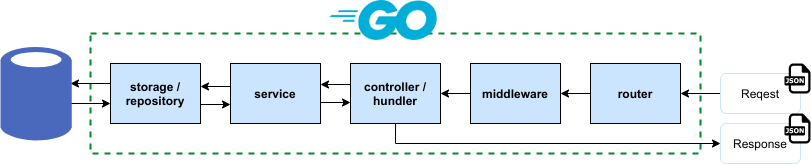
\includegraphics[width=1\linewidth]{rys03/backend_data_flow.png}
\caption{Przepływ danych}
\label{fig:backend_data_flow}
\end{figure}

% 
\subsubsection{Punkty końcowe}
Część serwerowa jest napisana zgodnie z modelem Rest API. Wymiana danymi zachodzi za pomocą standardów: HTTP (ang. \textit{HyperText Transfer Protocol}), URL, JSON.
W tabeli \ref{tab:endpoints} przedstawiony spis endpointów razem z metodą ich wysłania oraz krótkim opisem.
\begin{table}[htb] \small
    \caption{Lista Enpointów części serwerowej}
    \label{tab:endpoints}
    \begin{tabularx}{\linewidth}{| m{0.45cm} | m{1.5cm} | m{6cm} | X |}
    \hline
    № & Metoda & Endpoint & Opis \\
    \hline
    1 & GET & /api/v1 & Endpoint do testowania działania serwera. \\
    \hline
    2 & POST & /api/v1/login & Zalogowanie się użytkownika. \\
    \hline
    3 & GET & /api/v1/logout & Wylogowanie się użytkownika. \\
    \hline
    4 & POST & /api/v1/users & Tworzenie użytkownika. \\
    \hline
    5 & GET & /api/v1/users/{id} & Wczytywanie danych jednego użytkownika. \\
    \hline
    6 & PUT & /api/v1/users/{id} & Edycja użytkownika. \\
    \hline
    7 & DELETE & /api/v1/users/{id} & Usuwanie użytkownika. \\
    \hline
    8 & GET & /api/v1/users/read?skip=""\&limit="" & Wczytywanie danych limitowanej listy użytkowników użytkownika. \\
    \hline
    9 & POST & /api/v1/stations & Tworzenie stacji ładowniczej. \\
    \hline
    10 & GET & /api/v1/stations/{id} & Wczytywanie danych jednej stacji ładowniczej. \\
    \hline
    11 & PUT & /api/v1/stations/{id}?ownid="" & Edycja stacji. \\
    \hline
    12 & DELETE & /api/v1/stations/{id} & Usuwanie stacji ładowniczej. \\
    \hline
    13 & GET & /api/v1/stations/read?skip=""\&limit=""\&lat=""\&lng=""\&dist=""\&descr=""\&nam="" & Wyszukiwnaie stacji ładowniczej w zależności od parametrów. \\
    \hline
    14 & POST & /api/v1/stations/{sid}/comments & Tworzenie komentarza. \\
    \hline
    15 & GET & /api/v1/stations/{sid}/comments{id} & Wczytywanie danych jednego komentarza. \\
    \hline
    16 & PUT & /api/v1/stations/{sid}/comments{id} & Edycja komentarza. \\
    \hline
    17 & DELETE & /api/v1/stations/{sid}/comments{id} & Usuwanie komentarza. \\
    \hline
    18 & GET & /api/v1/stations/{sid}/read?skip=""\&limit="" & Wczytywanie danych limitowanej listy komentarzy należących do pewnej stacji. \\
    \hline
    \end{tabularx}
\end{table}

Kodem \ref{list:routers} została przedstawiona implementacja endpointów.
Dla rejestracji połączeń wchodzących zostanły użyte metody medialne \texttt{s.logger.SetRequestID} do przyznaczenia id każdemu połączniu oraz \texttt{s.logger.LogRequest} do wypisywania tego do konsoli.
Dla większości przypadków też jest sprawdzano czy jest użytkownik zalogowany do systemu \texttt{s.authController.CheckToken}. To będzie wyjaśnione później (sekcja \ref{sec:autentykacja}).
\begin{lstlisting}[label=list:routers,caption=Implementacja punktów końcowych,basicstyle=\tiny\ttfamily]
func (s *Server) SetupRouters() *mux.Router {
	v1 := "/api/v1"
	s.router.Schemes("http")
	s.router.Use(s.logger.SetRequestID) // middleware
	s.router.Use(s.logger.LogRequest)   // middleware
	s.router.HandleFunc(v1, s.testController.TestAPIV1()).Methods("GET")
	s.router.HandleFunc(v1+"/users", s.authController.CreateUser()).Methods("POST")
	s.router.HandleFunc(v1+"/login", s.authController.Login()).Methods("POST")
	s.router.HandleFunc(v1+"/logout/{id}", s.authController.Logout()).Methods("GET")

	user := s.router.PathPrefix(v1 + "/users").Subrouter()
	user.Use(s.authController.CheckToken)
	user.HandleFunc("/read", s.userController.Read()).Methods("GET")
	user.HandleFunc("/{id}", s.userController.FindByID()).Methods("GET")
	user.HandleFunc("/{id}", s.userController.DeleteByID()).Methods("DELETE")
	user.HandleFunc("/{id}", s.userController.UpdateByID()).Methods("PUT")

	stat := s.router.PathPrefix(v1 + "/stations").Subrouter()
	stat.Use(s.authController.CheckToken)
	stat.HandleFunc("", s.statController.CreateStation()).Methods("POST")
	stat.HandleFunc("/read", s.statController.Read()).Methods("GET")
	stat.HandleFunc("/{id}", s.statController.FindByID()).Methods("GET")
	stat.HandleFunc("/{id}", s.statController.DeleteByID()).Methods("DELETE")
	stat.HandleFunc("/{id}", s.statController.UpdateByID()).Methods("PUT")

	comm := stat.PathPrefix("/{sid}/comments").Subrouter()
	comm.Use(s.authController.CheckToken)
	comm.HandleFunc("/read", s.commController.Read()).Methods("GET")
	comm.HandleFunc("", s.commController.CreateComment()).Methods("POST")
	comm.HandleFunc("/{id}", s.commController.FindByID()).Methods("GET")
	comm.HandleFunc("/{id}", s.commController.DeleteByID()).Methods("DELETE")
	comm.HandleFunc("/{id}", s.commController.UpdateByID()).Methods("PUT")
	return s.router
}
\end{lstlisting}

% 
\subsection{Funkcje części serwerowej}
W tej sekcji są opisane implementacje endpointów części serwerowej.
% 
\subsubsection{Użytkownik}
Użytkownik jest niezbędny w pierwszej kolejności do uwierzytelniania. Niektóre dane użytkownika też są używane dla rozumienia: do kogo należy stacja ładownicza lub komentarz.

W listingu \ref{list:user_model} jest przedstawiona struktura użytkownika, wraz ze sposobem konwersji do JSON i BSON, która znajdująca się w pliku \texttt{models/user}.
\begin{lstlisting}[label=list:user_model,caption=Model danych użytkownika,basicstyle=\tiny\ttfamily]
    type User struct {
        ID       string `bson:"_id,omitempty" json:"_id,omitempty"`
        UserName string `bson:"user_name,omitempty" json:"user_name,omitempty"`
        Email    string `bson:"email,omitempty" json:"email,omitempty"`
        Password string `bson:"password,omitempty" json:"password,omitempty"`
        Model
    }
\end{lstlisting}

% 
% \paragraph{Dodawanie}\mbox{}\\
% Do tworzenia użytkownika został zaimplementowany endpoint \texttt{/api/v1/users}.
% Metoda zapytania \texttt{POST}.
% Jako ciało zapytania należy wysyłać obiekt w formacie JSON. Przykład:
% \begin{lstlisting}[basicstyle=\tiny\ttfamily]
%     {
%         "email": "email@test3.com",
%         "user_name": "test_user_1",
%         "password": "password"
%     }
% \end{lstlisting}
% Na serwerze nie sprawdza się, czy jest użytkownik już zalogowany, ponieważ ten endpoint również używany przy rejestracji.
% Zwraca JSON obiekt stworzonego użytkownika.

% Za pomocą routera jest realizowane przekierowanie z URL do wywołania metody kontrolera \texttt{CreateUser()} (listing \ref{list:user_controller_create}), w którym zaczyna się obróbka biznesowa zapytania.
% W tej metodzie są dekodowane dane z ciała zapytania, które są w formacie JSON, i przekazane do metody serwisu \texttt{CreateUser()} (listing \ref{list:user_service_create}). Po otrzymaniu danych z serwisu jest wysyłana odpowiedź.
% \begin{lstlisting}[label=list:user_controller_create,caption=Kontroler tworzenia użytkownika,basicstyle=\tiny\ttfamily]
%     func (c *UserController) CreateUser() http.HandlerFunc {
%         return http.HandlerFunc(func(w http.ResponseWriter, r *http.Request) {
%             u := &models.User{}
%             err := json.NewDecoder(r.Body).Decode(u)
%             if err != nil {
%                 utils.Error(w, r, http.StatusBadRequest, err)
%                 return
%             }
%             u, err = c.service.User().CreateUser(u)
%             if err != nil {
%                 utils.Error(w, r, http.StatusBadRequest, err)
%                 return
%             }
%             utils.Respond(w, r, http.StatusCreated, u)
%         })
%     }
% \end{lstlisting}

% W metodzie \texttt{CreateUser()} (listing \ref{list:user_service_create}) zachodzi:
% \begin{itemize}
%     \item walidacja danych;
%     \item sprawdzanie, czy istnieje użytkownik z taką pocztą mailową;
%     \item jeśli nie istnieje, to zachodzi szyfrowanie hasła oraz ustalenie czasu tworzenia i edycji obiektu. Jeśli już istnieje, to zwraca błąd;
%     \item tworzenie nowego użytkownika w bazie danych;
%     \item przygotowanie obiektu użytkownika do transmisji: usuwanie hasła i daty tworzenia dla bezpieczeństwa oraz szybkości transmisji danych.
% \end{itemize}
% Ta metoda znajduje się w pliku \texttt{services/v1/userservice.go}.
% \begin{lstlisting}[label=list:user_service_create,caption=Serwis tworzenia użytkownika,basicstyle=\tiny\ttfamily]
%     func (s *UserService) CreateUser(u *models.User) (*models.User, error) {
%         if err := u.Validate(); err != nil {
%             return u, err
%         }
%         _, err := s.storage.User().FindByEmail(u.Email)
%         if err != utils.ErrRecordNotFound {
%             if err != nil {
%                 return nil, err
%             }
%             return u, utils.ErrRecordAlreadyExists
%         }
%         if err := u.BeforeCreate(); err != nil {
%             return u, err
%         }
%         id, err := s.storage.User().Create(u)
%         if err != nil {
%             return nil, err
%         }
%         u, err = s.storage.User().FindByID(id)
%         if err != nil {
%             return nil, err
%         }
%         u.Sanitize()
%         return u, nil
%     }
% \end{lstlisting}

% Metoda \texttt{Create()} (listing \ref{list:user_repository_create}) tworzy zapis nowego użytkownika w bazie danych i zwraca jego ID.
% Ona znajduję się w \texttt{/storage/mongostore/userrepository.go}.
% \begin{lstlisting}[label=list:user_repository_create,caption=Zachowanie użytkownika do bazy danych,basicstyle=\tiny\ttfamily]
%     func (r *UserRepository) Create(u *models.User) (string, error) {
%         res, err := r.col.InsertOne(context.TODO(), u)
%         if err != nil {
%             return "", err
%         }
%         id := res.InsertedID.(primitive.ObjectID).Hex()
%         return id, nil
%     }
% \end{lstlisting}

% 
\paragraph{Wczytywanie}\mbox{}\\

Do wczytywania konkretnego użytkownika został zaimplementowany endpoint \texttt{/api/v1/users/{id}}.
Metoda zapytania \texttt{GET}.
W adresie URL musi być podany id użytkownika.
Dla korzystania z danego endpointu użytkownik musi być zalogowany.
Zwraca JSON obiekt znalezionego użytkownika.

Za pomocą routera jest realizowane przekierowanie z URL do wywołania metody kontrolera użytkownika \texttt{FindByID()} (listing \ref{list:user_controller_findbyid}), która zaczyna obróbkę biznesową zapytania.
W tej metodzie jest wywoływana metoda serwisu \texttt{FindByID()} (listing \ref{list:user_service_findbyid}). Później jest wysyłana odpowiedź.
\begin{lstlisting}[label=list:user_controller_findbyid,caption=Kontroler wczytywania użytkownika,basicstyle=\tiny\ttfamily]
    func (c *UserController) FindByID() http.HandlerFunc {
        return http.HandlerFunc(func(w http.ResponseWriter, r *http.Request) {
            params := mux.Vars(r)
            id, ok := params["id"]
            if !ok {
                utils.Error(w, r, http.StatusBadRequest, utils.ErrWrongRequest)
                return
            }
            u, err := c.service.User().FindByID(id)
            if err != nil {
                utils.Error(w, r, http.StatusNoContent, err)
                return
            }
            utils.Respond(w, r, http.StatusFound, u)
        })
    }
\end{lstlisting}
% 
Metoda \texttt{FindByID()} (listing \ref{list:user_service_findbyid}) z pliku \texttt{services/v1/userservice.go}:
\begin{lstlisting}[label=list:user_service_findbyid,caption=Serwis wczytywania użytkownika,basicstyle=\tiny\ttfamily]
    func (s *UserService) FindByID(id string) (*models.User, error) {
        u, err := s.storage.User().FindByID(id)
        if err != nil {
            return nil, err
        }
        u.Sanitize()
        return u, nil
    }
\end{lstlisting}
% 
Metoda \texttt{FindByID()} (listing \ref{list:user_repository_findbyid}) wyszukuje użytkownika z pewnym ID w bazie dabych.
Ona znajduję się w \texttt{/storage/mongostore/userrepository.go}.
\begin{lstlisting}[label=list:user_repository_findbyid,caption=Wczytywanie uzytkownika z bazy danych,basicstyle=\tiny\ttfamily]
    func (r *UserRepository) FindByID(id string) (*models.User, error) {
        idi, err := primitive.ObjectIDFromHex(id)
        if err != nil {
            return nil, err
        }
        filter := bson.M{"_id": idi}
        res := r.col.FindOne(context.TODO(), filter)
        u := &models.User{}
        err = res.Decode(u)
        if err != nil {
            return nil, utils.ErrRecordNotFound
        }
        return u, nil
    }
\end{lstlisting}

% 
\paragraph{Edycja}\mbox{}\\

Do edycji użytkownika został zaimplementowany endpoint \texttt{/api/v1/users/{id}}.
Metoda zapytania \texttt{PUT}.
W adresie URL musi być podany id użytkownika.
Jako ciało zapytania należy wysyłać obiekt w formacie JSON. Przykład:
\begin{lstlisting}[basicstyle=\tiny\ttfamily]

    {
        "user_name": "test_user_2",
        "update_at": "2020-11-01T13:27:31.105Z"
    }
\end{lstlisting}
Dla korzystania z danego endpointu użytkownik musi być zalogowany.

Za pomocą routera jest realizowane przekierowanie z URL do wywołania metody kontrolera użytkownika \texttt{UpdateByID()} (listing \ref{list:user_controller_UpdateByID}), która zaczyna obróbkę biznesową zapytania.
W tej metodzie jest wywoływana metoda serwisu \texttt{UpdateByID()} (listing \ref{list:user_service_UpdateByID}). Później jest wysyłana odpowiedź.
\begin{lstlisting}[label=list:user_controller_UpdateByID,caption=Kontroler edycji użytkownika,basicstyle=\tiny\ttfamily]
    func (c *UserController) UpdateByID() http.HandlerFunc {
        return http.HandlerFunc(func(w http.ResponseWriter, r *http.Request) {
            params := mux.Vars(r)
            id, ok := params["id"]
            if !ok {
                utils.Error(w, r, http.StatusNoContent, utils.ErrWrongRequest)
                return
            }
            u := &models.User{}
            err := json.NewDecoder(r.Body).Decode(u)
            if err != nil {
                utils.Error(w, r, http.StatusBadRequest, err)
                return
            }
            u, err = c.service.User().UpdateByID(id, u)
            if err != nil {
                utils.Error(w, r, http.StatusNotFound, err)
                return
            }
            utils.Respond(w, r, http.StatusOK, u)
        })
    }
\end{lstlisting}
% % 
Metoda \texttt{UpdateByID()} (listing \ref{list:user_service_UpdateByID}) z pliku \texttt{services/v1/userservice.go}:
\begin{lstlisting}[label=list:user_service_UpdateByID,caption=Serwis edycji użytkownika,basicstyle=\tiny\ttfamily]
    func (s *UserService) UpdateByID(id string, u *models.User) (*models.User, error) {
        if u.Password != "" {
            tmp, err := models.EncryptString(u.Password)
            u.Password = tmp
            if err != nil {
                return nil, err
            }
        }
        err := s.storage.User().UpdateByID(id, u)
        if err != nil {
            return nil, err
        }
        u, err = s.storage.User().FindByID(id)
        if err != nil {
            return nil, err
        }
        u.Sanitize()
        return u, nil
    }
\end{lstlisting}
% % 
Metoda \texttt{UpdateByID()} (listing \ref{list:user_repository_UpdateByID}) wyszukuje i aktualizuje użytkownika z pewnym ID i \texttt{update\_at} w bazie dabych.
Ona znajduję się w \texttt{/storage/mongostore/userrepository.go}.
\begin{lstlisting}[label=list:user_repository_UpdateByID,caption=Edycja uzytkownika w bazie danych,basicstyle=\tiny\ttfamily]
    func (r *UserRepository) UpdateByID(id string, u *models.User) error {
        idi, err := primitive.ObjectIDFromHex(id)
        if err != nil {
            return err
        }
        filter := bson.M{
            "_id":             idi,
            "model.update_at": u.UpdateAt,
        }
        update := bson.M{
            "model.update_at": models.GetTimeNow(),
        }
        if u.UserName != "" {
            update["user_name"] = u.UserName
        }
        if u.Email != "" {
            update["email"] = u.Email
        }
        if u.Password != "" {
            update["password"] = u.Password
        }
        _, err = r.col.UpdateOne(context.TODO(), filter, bson.M{
            "$set": update})
        if err != nil {
            return err
        }
        return nil
    }
\end{lstlisting}

% % 
\paragraph{Usunięcie}\mbox{}\\

Do Usunięcia użytkownika został zaimplementowany endpoint \texttt{/api/v1/users/{id}}.
Metoda zapytania \texttt{DELETE}.
W adresie URL musi być podany id użytkownika.

Dla korzystania z danego endpointu użytkownik musi być zalogowany.

Za pomocą routera jest realizowane przekierowanie z URL do wywołania metody kontrolera użytkownika \texttt{DeleteByID()} (listing \ref{list:user_controller_DeleteByID}), która zaczyna obróbkę biznesową zapytania.
W tej metodzie jest wywoływana metoda serwisu \texttt{DeleteByID()} (listing \ref{list:user_service_DeleteByID}). Później jest wysyłana odpowiedź.
\begin{lstlisting}[label=list:user_controller_DeleteByID,caption=Kontroler usunięcia użytkownika,basicstyle=\tiny\ttfamily]
    func (c *UserController) DeleteByID() http.HandlerFunc {
        return http.HandlerFunc(func(w http.ResponseWriter, r *http.Request) {
            params := mux.Vars(r)
            id, ok := params["id"]
            if !ok {
                utils.Error(w, r, http.StatusBadRequest, utils.ErrWrongRequest)
                return
            }
            err := c.service.User().DeleteByID(id)
            if err != nil {
                utils.Error(w, r, http.StatusNoContent, err)
                return
            }
            utils.Respond(w, r, http.StatusOK, nil)
        })
    }
\end{lstlisting}
% % 
Metoda \texttt{DeleteByID()} (listing \ref{list:user_service_DeleteByID}) z pliku \texttt{services/v1/userservice.go}:
\begin{lstlisting}[label=list:user_service_DeleteByID,caption=Serwis usunięcia użytkownika,basicstyle=\tiny\ttfamily]
    func (s *UserService) DeleteByID(id string) error {
        return s.storage.User().DeleteByID(id)
    }
\end{lstlisting}
% 
Metoda \texttt{DeleteByID()} (listing \ref{list:user_repository_DeleteByID}) usuwa użytkownika z pewnym ID z bazy dabych.
Ona znajduję się w \texttt{/storage/mongostore/userrepository.go}.
\begin{lstlisting}[label=list:user_repository_DeleteByID,caption=Usunięcie uzytkownika z bazy danych,basicstyle=\tiny\ttfamily]
    func (r *UserRepository) DeleteByID(id string) error {
        idi, err := primitive.ObjectIDFromHex(id)
        if err != nil {
            return err
        }
        filter := bson.M{"_id": idi}
        res, err := r.col.DeleteOne(context.TODO(), filter)
        if err != nil {
            return err
        }
        if res.DeletedCount == 0 {
            return utils.ErrRecordNotFound
        }
        return nil
    }
\end{lstlisting}

\subsubsection{Autentykacja / Logowanie i rejestracja}
\label{sec:autentykacja}
Dla autentykacji został wykorzystany JWT token, który jest generowany na serwerze, przy znalezieniu użytkownika o podanym adresie mailowym i haśle w bazie danych, i za tym jest wysłany w nagłówku odpowiedzi razem z danymi tego użytkownika.
Ten token jest ważny jeden tydzień, za tym traci ważność i należy zalogować się ponownie. Wewnątrz tokena znajduje się nagłówek, sygnatura, czas ważności i id użytkownika.
Większość endpointów dostępny tylko dla uwierzytelnionych użytkowników. W nagłówku zapytania musi znajdować się ważny token oraz ten token nie musi znajdować się na czarnej liście tokenów przechowywanych w bazie danych Redis.

\paragraph{Logowanie\newline}
Dla zalogowania należy wysłać metodą POST zapytanie na endpoint \texttt{api/v1/login} z ciałem zawierającym \texttt{email} i \texttt{password} w formacie JSON:
\begin{lstlisting}[basicstyle=\tiny\ttfamily]
    {
        "email": "test@test.test",
        "password": "password"
    }
\end{lstlisting}

Mapowanie routera przekieruje to zapytanie do metody \texttt{Login()}, która się znajduje w \texttt{controllers/api/authcontroller.go} \ref{list:authcontroller_login}.
W tej metodzie, po znalezieniu użytkownika o takim adresie mailowym i hasle (\ref{list:authcontroller_login}), jest generowany token JWT (\ref{list:get_jwt_token}) i wysyła się odpowidż zawierająca nagłówek z tokenem oraz ciało z danymi użytkownika.
\begin{lstlisting}[label=list:authcontroller_login,caption=Kontroller logowania użytkownika,basicstyle=\tiny\ttfamily]
    func (c *AuthController) Login() http.HandlerFunc {
        return http.HandlerFunc(func(w http.ResponseWriter, r *http.Request) {
            u := &models.User{}
            err := json.NewDecoder(r.Body).Decode(u)
            if err != nil {
                utils.Error(w, r, http.StatusBadRequest, err)
                return
            }
            u, err = c.service.User().Login(u)
            if err != nil {
                utils.Error(w, r, http.StatusUnauthorized, utils.ErrIncorrectEmailOrPassword)
                return
            }
            token, err := c.createTokenString(u.ID)
            if err != nil {
                utils.Error(w, r, http.StatusInternalServerError, err)
                return
            }
            w.Header().Set("Authorization", "Bearer "+token)
            utils.Respond(w, r, http.StatusOK, u)
        })
    }
\end{lstlisting}

\begin{lstlisting}[label=list:get_jwt_token,caption=Generacja JWT tokena,basicstyle=\tiny\ttfamily]
    func (c *AuthController) createTokenString(uid string) (string, error) {
        expirationTime := time.Now().Add(168 * time.Hour)
        claims := &Claims{
            UID: uid, // user id
            StandardClaims: jwt.StandardClaims{
                ExpiresAt: expirationTime.Unix(), //lifetime
            },
        }
        token := jwt.NewWithClaims(jwt.SigningMethodHS256, claims)
        tokenString, err := token.SignedString([]byte(c.jwtKey))
        if err != nil {
            return "", err
        }
        return tokenString, nil
    }
\end{lstlisting}

Dla wyszukiwania użytkownika o podanym adresie mailowym i haśle jest używana metoda \texttt{Login} (\ref{list:userservice_login}) znajdująca się w \texttt{serwices/api/v1/userservice.go},
która wyszukuje w bazie danych użytkownika o podanym adresie (adresy mailowe są unikalne) za pomocą metody \texttt{FindByEmal()} (\ref{list:userrepository_findbyemail}) z pliku \texttt{storage/mongostore/userrepository.go} i porównuje hashowane hasło, z bazy danych, z nie haszowanym, z zapytania (\ref{list:validate_password}).
\begin{lstlisting}[label=list:userservice_login,caption=Serwis logowania uzytkownika,basicstyle=\tiny\ttfamily]
    func (s *UserService) Login(u *models.User) (*models.User, error) {
        if err := u.Validate(); err != nil {
            return nil, err
        }
        u2, err := s.storage.User().FindByEmail(u.Email)
        if err != nil {
            return nil, err
        }
        if !u2.VerifyPassword(u.Password) {
            return nil, utils.ErrIncorrectEmailOrPassword
        }
        u2.Sanitize()
        return u2, nil
    }
\end{lstlisting}

\begin{lstlisting}[label=list:userrepository_findbyemail,caption=Wysukiwanie użytkownika w bazie po adresie mailowym,basicstyle=\tiny\ttfamily]
    func (r *UserRepository) FindByEmail(email string) (*models.User, error) {
        filter := bson.M{"email": email}
        res := r.col.FindOne(context.TODO(), filter)
        u := &models.User{}
        err := res.Decode(u)
        if err != nil {
            return nil, utils.ErrRecordNotFound
        }
        return u, nil
    }
\end{lstlisting}

\begin{lstlisting}[label=list:validate_password,caption=Porównywanie hasła,basicstyle=\tiny\ttfamily]
    func (u *User) VerifyPassword(p string) bool {
        return bcrypt.CompareHashAndPassword([]byte(u.Password), []byte(p)) == nil
    }
\end{lstlisting}

\paragraph{Rejestracja\newline}
Aby zarejestrować nowego użytkownika, należy wysłać zapytanie POST na adres \texttt{api/v1/users} z odpowiednim ciałem JSON:
\begin{lstlisting}[basicstyle=\tiny\ttfamily]
    {
        "email": "email@test3.com",
        "user_name": "test_user_1",
        "password": "password"
    }
\end{lstlisting}

Dalej zostanie wykonana metoda \texttt{CreateUser()} z pliku \texttt{controllers/api/v1/authcontroller.go} \ref{list:user_controller_create}.
W tej metodzie są dekodowane dane z ciała zapytania, które są w formacie JSON, i przekazane do metody \texttt{CreateUser()} (listing \ref{list:user_service_create}), która znajduje się w pliku \texttt{services/api/v1/userservice.go}. Po otrzymaniu danych z serwisu jest tworzony token oraz wysyłana odpowiedź, która zawiera wygenerowany token i dane utworzonego użytkownika.
\begin{lstlisting}[label=list:user_controller_create,caption=Kontroler tworzenia użytkownika,basicstyle=\tiny\ttfamily]
    func (c *UserController) CreateUser() http.HandlerFunc {
        return http.HandlerFunc(func(w http.ResponseWriter, r *http.Request) {
            u := &models.User{}
            err := json.NewDecoder(r.Body).Decode(u)
            if err != nil {
                utils.Error(w, r, http.StatusBadRequest, err)
                return
            }
            u, err = c.service.User().CreateUser(u)
            if err != nil {
                utils.Error(w, r, http.StatusBadRequest, err)
                return
            }
            utils.Respond(w, r, http.StatusCreated, u)
        })
    }
\end{lstlisting}

W metodzie \texttt{CreateUser()} (listing \ref{list:user_service_create}) zachodzi:
\begin{itemize}
    \item walidacja danych;
    \item sprawdzanie, czy istnieje użytkownik z taką pocztą mailową;
    \item jeśli nie istnieje, to zachodzi haszowanie hasła \ref{list:hash_pass} oraz ustalenie czasu tworzenia i edycji obiektu. Jeśli już istnieje, to zwraca błąd;
    \item tworzenie nowego użytkownika w bazie danych;
    \item przygotowanie obiektu użytkownika do transmisji: usuwanie hasła i daty tworzenia dla bezpieczeństwa oraz szybkości transmisji danych.
\end{itemize}
Ta metoda znajduje się w pliku \texttt{services/api/v1/userservice.go}.
\begin{lstlisting}[label=list:user_service_create,caption=Serwis tworzenia użytkownika,basicstyle=\tiny\ttfamily]
    func (s *UserService) CreateUser(u *models.User) (*models.User, error) {
        if err := u.Validate(); err != nil {
            return u, err
        }
        _, err := s.storage.User().FindByEmail(u.Email)
        if err != utils.ErrRecordNotFound {
            if err != nil {
                return nil, err
            }
            return u, utils.ErrRecordAlreadyExists
        }
        if err := u.BeforeCreate(); err != nil {
            return u, err
        }
        id, err := s.storage.User().Create(u)
        if err != nil {
            return nil, err
        }
        u, err = s.storage.User().FindByID(id)
        if err != nil {
            return nil, err
        }
        u.Sanitize()
        return u, nil
    }
\end{lstlisting}
\begin{lstlisting}[label=list:hash_pass,caption=Haszowanie hasła,basicstyle=\tiny\ttfamily]
    func EncryptString(str string) (string, error) {
        b, err := bcrypt.GenerateFromPassword([]byte(str), bcrypt.MinCost)
        if err != nil {
            return "", err
        }
        return string(b), nil
    }
\end{lstlisting}

Metoda \texttt{Create()} (listing \ref{list:user_repository_create}) tworzy zapis nowego użytkownika w bazie danych i zwraca jego ID.
Ona znajduję się w \texttt{/storage/mongostore/userrepository.go}.
\begin{lstlisting}[label=list:user_repository_create,caption=Zachowanie użytkownika do bazy danych,basicstyle=\tiny\ttfamily]
    func (r *UserRepository) Create(u *models.User) (string, error) {
        res, err := r.col.InsertOne(context.TODO(), u)
        if err != nil {
            return "", err
        }
        id := res.InsertedID.(primitive.ObjectID).Hex()
        return id, nil
    }
\end{lstlisting}

\paragraph{Sprawdzenie tokenu\newline}
Większość, jak juz zostało powiedziano, endpointów pracują tylko z uwierzytelnionymi użytkownikami. Dla realizacji tej funkcji należy sprawdzić token, który zawiera nagłówek zapytania.
Token musi nie tylko nie stracić ważności, ale i nie znajdować się w czarnej liście tokenów, która znajduje się Redis, bazie danych wykonującej rolę pamięci podręcznej.
Metoda \texttt{CheckToken()} sprawdza te rzeczy (\ref{list:CheckToken}).
\begin{lstlisting}[label=list:CheckToken,caption=Walidacja JWT tokenu,basicstyle=\tiny\ttfamily]
    func (c *AuthController) CheckToken(next http.Handler) http.Handler {
        return http.HandlerFunc(func(w http.ResponseWriter, r *http.Request) {
            tokenString := r.Header.Get("Authorization")
            if len(tokenString) == 0 {
                utils.Error(w, r, http.StatusUnauthorized, errors.New("Missing Authorization Header"))
                return
            }
            tokenString = strings.Replace(tokenString, "Bearer ", "", 1)
            claims := &Claims{}
            tkn, err := jwt.ParseWithClaims(tokenString, claims, func(token *jwt.Token) (interface{}, error) {
                return []byte(c.jwtKey), nil
            })
            if err != nil {
                if err == jwt.ErrSignatureInvalid {
                    utils.Error(w, r, http.StatusUnauthorized, err)
                    return
                }
                utils.Error(w, r, http.StatusBadRequest, err)
                return
            }
            if !tkn.Valid {
                utils.Error(w, r, http.StatusUnauthorized, err)
                return
            }
            _, err = c.rClient.Get(tokenString[37:]).Result() // find tocken in Redis
            if err != redis.Nil {
                utils.Error(w, r, http.StatusUnauthorized, errors.New("Invalid token"))
                return
            }
            next.ServeHTTP(w, r)
        })
    }
\end{lstlisting}

\paragraph{Wylogowanie\newline}
Po wysłaniu zapytania GET na adres \texttt{api/v1/logout}, zostanie wywoływana metoda \texttt{Logout()} (\ref{list:logout}) podczas działania której zostanie sprawdzony token (\ref{list:CheckToken}), za tym dodany do bazy danych Redis (pamięci podręcznej) oraz usunięty z nagłówka odpowiedzi.
\begin{lstlisting}[label=list:logout,caption=Wylogowanie,basicstyle=\tiny\ttfamily]
    func (c *AuthController) Logout() http.HandlerFunc {
        return http.HandlerFunc(func(w http.ResponseWriter, r *http.Request) {
            tokenString := r.Header.Get("Authorization")
            if len(tokenString) == 0 {
                utils.Error(w, r, http.StatusUnauthorized, errors.New("Missing Authorization Header"))
                return
            }
            tokenString = strings.Replace(tokenString, "Bearer ", "", 1)
            claims := &Claims{}
            tkn, err := jwt.ParseWithClaims(tokenString, claims, func(token *jwt.Token) (interface{}, error) {
                return []byte(c.jwtKey), nil
            })
            if err != nil {
                if err == jwt.ErrSignatureInvalid {
                    utils.Error(w, r, http.StatusUnauthorized, err)
                    return
                }
                utils.Error(w, r, http.StatusBadRequest, err)
                return
            }
            if !tkn.Valid {
                utils.Error(w, r, http.StatusUnauthorized, err)
                return
            }
            _, err = c.rClient.Get(tokenString[37:]).Result() // find in Redis db
            if err != redis.Nil {
                utils.Error(w, r, http.StatusUnauthorized, errors.New("Invalid token"))
                return
            }
            params := mux.Vars(r)
            uid, ok := params["id"]
            if !ok {
                utils.Error(w, r, http.StatusBadRequest, utils.ErrWrongRequest)
                return
            }
            if uid != claims.UID {
                utils.Error(w, r, http.StatusBadRequest, utils.ErrWrongRequest)
                return
            }
            c.rClient.Set(tokenString[37:], tokenString, 168*time.Hour) // save to Redis db
            utils.Respond(w, r, http.StatusOK, nil)
        })
    }
\end{lstlisting}

\subsubsection{Stacja}
Głównym przedmiotem w aplikacji jest stacja ładująca pojazy elektryczne. Aplikacja została stworzona, aby uzyskać informacje o nich. Stacje można tworzyć, przeglądać, a także, jeśli użytkownik jest właścicielem, może je modyfikować.

W listingu \ref{list:station_model} jest przedstawiona struktura encji stacji ładowniczej, wraz ze sposobem konwersji do JSON i BSON, która znajdująca się w pliku \texttt{models/user}.
\begin{lstlisting}[label=list:station_model,caption=Model danych stacji ładowniczej,basicstyle=\tiny\ttfamily]
    type Station struct {
        ID          string    `bson:"_id,omitempty" json:"_id,omitempty"`
        StationName string    `bson:"station_name,omitempty" json:"station_name,omitempty"`
        OwnerID     string    `bson:"owner_id,omitempty" json:"owner_id,omitempty"`
        Rating      float32   `bson:"rating,truncate" json:"rating,truncate"`
        Description string    `bson:"description,omitempty" json:"description,omitempty"`
        Comments    []Comment `bson:"comments,omitempty" json:"comments,omitempty"`
        Latitude    float64   `bson:"latitude" json:"latitude"`
        Longitude   float64   `bson:"longitude" json:"longitude"`
        Model
    }
\end{lstlisting}

\paragraph{Dodawanie}
Żeby dodać nową stację do systemu należy wysłać zapytanie \testtt{POST} do części serwerowj na endpoint \texttt{api/v1/stations}. Zapytanie musi posiadać działający token JWT w nagłówku. Ciało zapytania musi posiadać następujące pola: \textt{description}, \textt{station_name}, \textt{owner_id}, \textt{longitude}, \textt{latitude}.
Przykład ciałą zapytania:
\begin{lstlisting}[basicstyle=\tiny\ttfamily]
    {
		"description": "testText",
		"station_name": "station name",
		"owner_id": "5fbe4b1a187e72c56a5e4f70",
		"longitude":    15.162,
		"latitude": 12.46
    }
\end{lstlisting}

Router przekieruje, po przechodzeniu przez funkcje medyalne, w tym sprawdzenie JWT tokenu, dane do kontrolera \textt{CreateStation()} \ref{list:} (plik \texttt{controllers/api/v1/stationcontoller.go}) który dekoduje wchodzący JSON w obiekt struktury \texttt{station}.
Ta metoda wywołuje serwis \texttt{CreateStation} \ref{list:}, znajdującyj się w pliku \texttt{services/api/v1/stationservice.go}, w którym sprawdza się czy istnieje stacja w tym mijscu, tworzy stację w bazie danych (metoda \texttt{Create} \ref{list:} z pliku \texttt{storage/mongostore/stationrepository.go}) oraz, przy udanym wpisie, pobiera z bazy danych ten dokumenty (listing \ref) i wysyła sie jako ciało odpowiedzi.




\paragraph{Wczytywanie}
\paragraph{Edycja}
\paragraph{Usunięcie}
\subsubsection{Komentarz}
\paragraph{Dodawanie}
\paragraph{Wczytywanie}
\paragraph{Edycja}
\paragraph{Usunięcie}
%
\section{Implementacja Intefejsu użytkownika}
\subsection{Struktura AndroidUI}
\subsubsection{Struktura plików AndroidUI}
\subsubsection{Przepływ danych}
\subsubsection{Nażędzia i technologie}
\subsection{Funkcje aplikacji mobilnej}
\subsubsection{Autentykacja / Logowanie i rejestracja}
\subsubsection{Stacja}
\paragraph{Dodawanie}
\paragraph{Wczytywanie}
\paragraph{Edycja}
\subsubsection{Komentarz}
\paragraph{Dodawanie}
\paragraph{Wczytywanie}
